\subsection*{Task 4}

\subsubsection*{a)}

The new objective function with regularization is

\begin{equation*}
  J(w) = C(w) + \lambda R(w), \quad\quad R(w) = ||w||^2 = \sum_{i,j} w_{i,j}^2,
\end{equation*}
where $C(w)$ is defined by \cref{eq:softmax_entropy}. The new gradient for the backward pass is then

\begin{align*}
  \frac{\partial J^n(w)}{\partial w_{kj}} &= \frac{1}{N} \sum_{n=1}^{N} \frac{\partial C^n(w)}{\partial w_{kj}} + \frac{\partial R(w)}{\partial w_{kj}} \\
                                          &= -\frac{1}{N} \sum_{n=1}^{N} x_j^n (y_k^n - \hat{y}_k^n) + 2 \lambda w_{kj}
\end{align*}



\subsubsection*{b)}

\begin{figure}[!h]
    \centering
    \begin{subfigure}[b]{\linewidth}
        \centering
        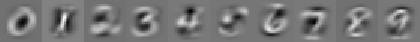
\includegraphics[width=\linewidth]{figures/Task4b_lambda0.pdf}
    \end{subfigure}
    \begin{subfigure}[b]{\linewidth}
        \centering
        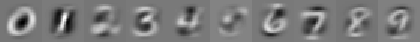
\includegraphics[width=\linewidth]{figures/Task4b_lambda1.pdf}
    \end{subfigure}
    \caption{Weights for model with $\lambda=0$ (top row) and $\lambda=1$ (bottom row).}
    \label{fig:task4:weights}
\end{figure}

In \cref{fig:task4:weights} we see the weights without regularization (top row) and with regularization (bottom row). Although the difference isn't as apparent as in the assignment text, we see that the bottom row is slightly more smoothed out. This is because the weights are overall smaller in value for the regularized model, as we in a sense have penalized the use of larger weights by the parameter $\lambda$. For the unregularized model there is no constraint on the magnitude of the weights, leading to possibly large contrasts between large and low values, which gives a more "noisy" image.
\newpage
\subsubsection*{c)}

\begin{figure}[h!]
  \centering
  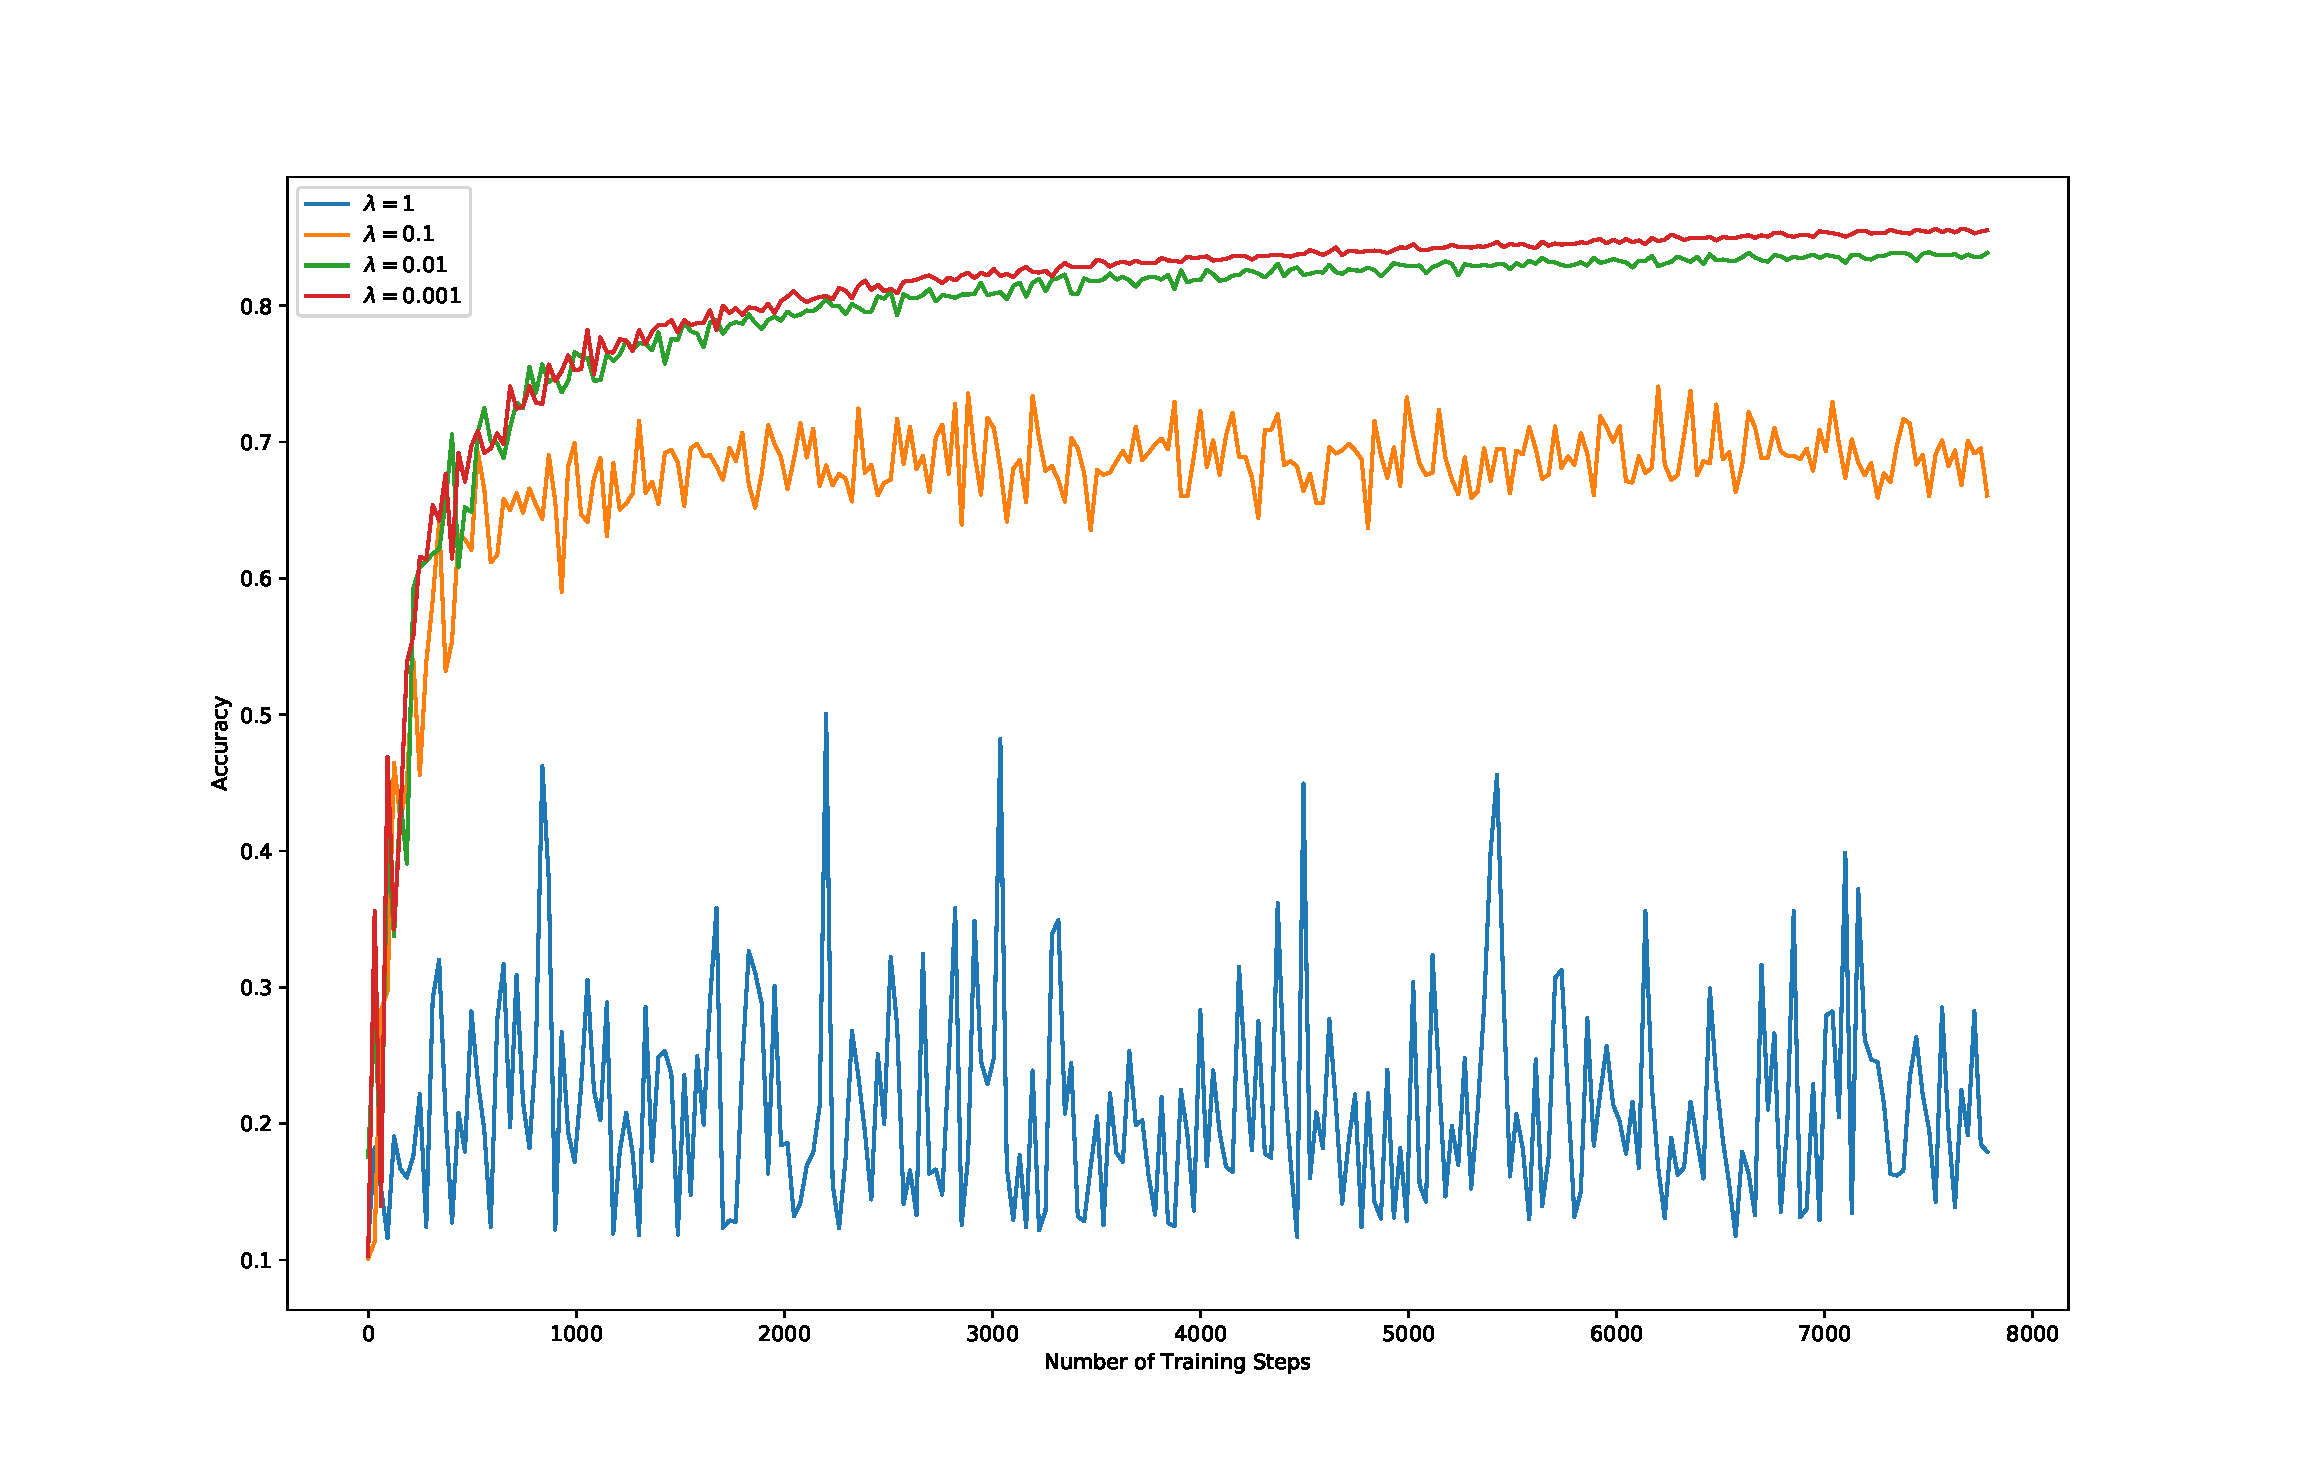
\includegraphics[clip, trim=0cm 0cm 0cm 0cm, width=\textwidth]{figures/Task4c.pdf}
  \caption{Validation set accuracy for different $\lambda$.}
  \label{fig:task4:val_accuracy_lambdas}
\end{figure}


\subsubsection*{d)}

From \cref{fig:task4:val_accuracy_lambdas} we see that the validation set accuracy degrades with increased regularization. I think this somewhat goes against the intentions of regularizing the model, as we use regularization for better generalization, which should give decent performance on the validation set. It may however be the case that the model is simple enough as it is, and by penalizing the complexity we get a so simple model that we underfit the data.


\subsubsection*{e)}

\begin{figure}[h!]
  \centering
  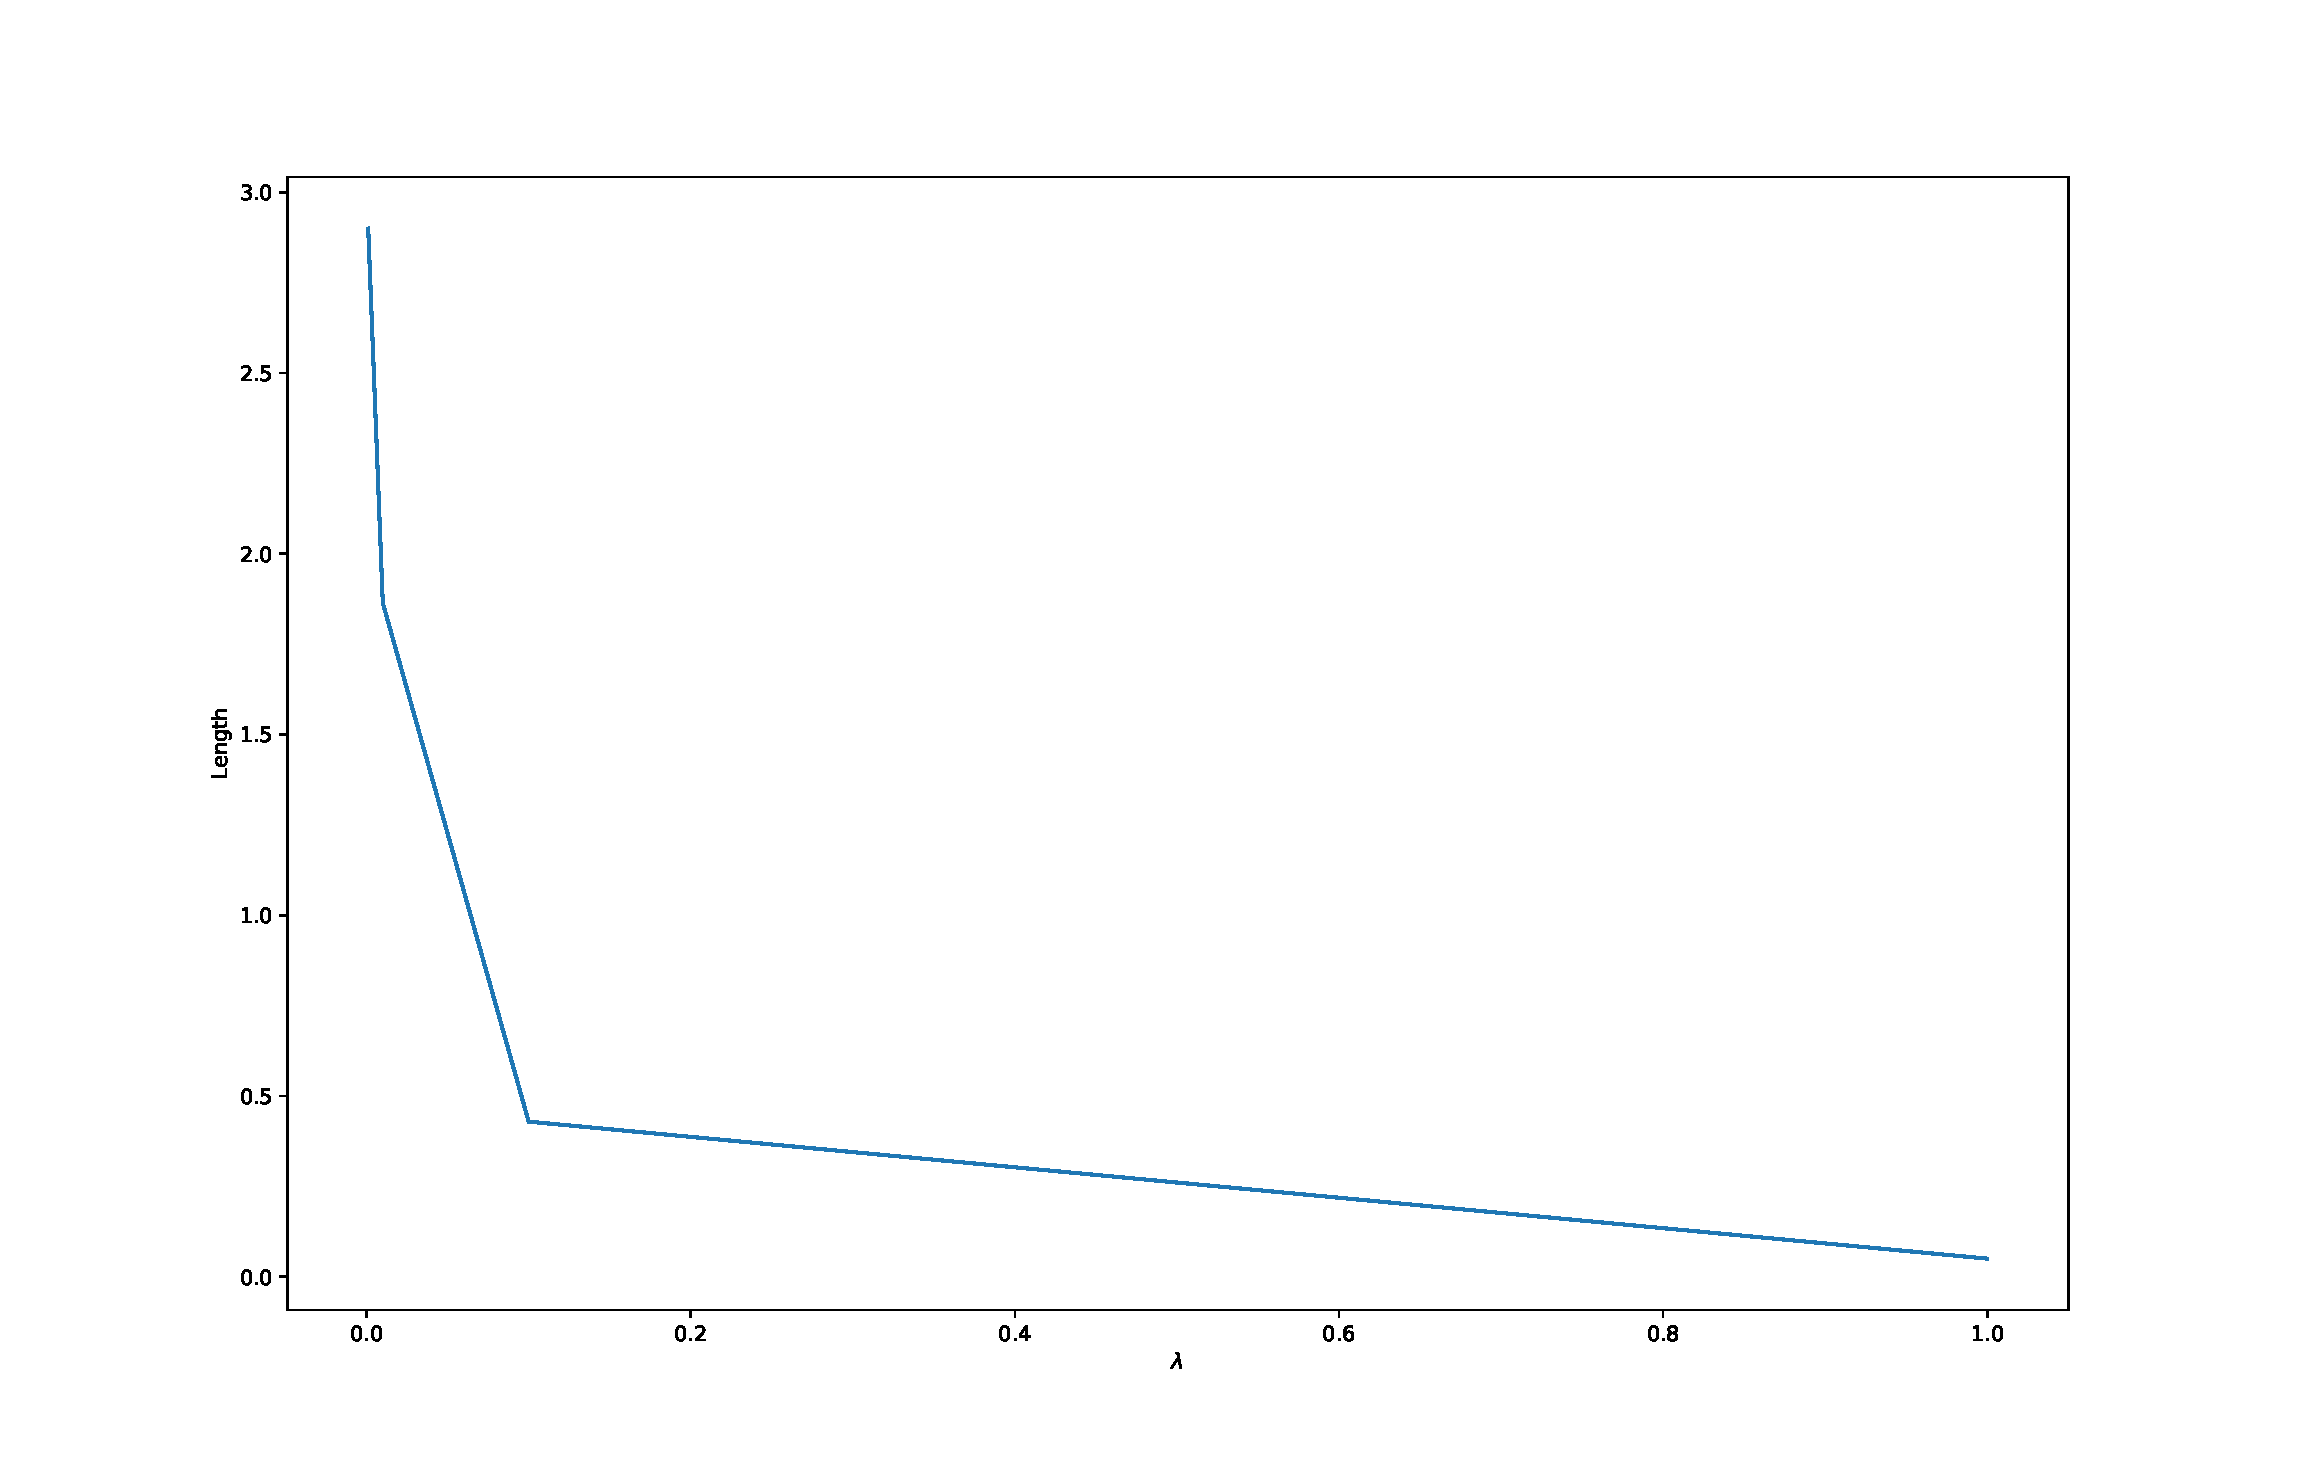
\includegraphics[clip, trim=0cm 0cm 0cm 0cm, width=\textwidth]{figures/Task4e.pdf}
  \caption{$L_2$ norm of weight vector $w$ for different $\lambda$.}
  \label{fig:task4:norm}
\end{figure}

From \cref{fig:task4:norm} we see that the length decreases with increasing $\lambda$, meaning the average values of $w$ decrease. This is evidence that regularization penalizes the weights, leading to simpler models.
